\subsection{DOP 28 Потоки в сетях. Алгоритм построения максимального потока. Оценка сложности алгоритма.}


\begin{itemize}
    \item \textbf{Потоковая сеть} --- набор $G = (V, E, c, s, t)$, где $(V, E)$ --- орграф без множественных дуг (в частности, $(u,v) \in E \implies (v, u) \notin E$), $c$ --- вектор пропускных способностей дуг, $|c| = |E|$, вершины $s, t$ --- исток и сток соответственно. Для каждой вершины $u$ обозначим:
    $$ u_+ = \{v \in V~|~(u, v) \in E\}$$
    $$u_- = \{v \in V~|~(v, u) \in E\}$$
    \item $f$ --- \textbf{поток} в $G$, т.е. вектор, $|f| = |E|$, для которого выполнены условия:
    \begin{enumerate}
        \item $f(e) \in [0, c(e)], e \in E$
        \item $\forall u \in V \setminus\{s, t\}$, $f_+(u) = \sum_{v \in u_+} f(u, v) = \sum_{v \in u_-} f (v, u) = f_-(u)$.
    \end{enumerate}
    \item $||f|| = f_+(s)$ --- \textbf{величина потока} в сети.
    \item \textbf{Задача поиска максимального потока:}
    Найти поток $f$ максимальной величины при условиях 1., 2.
\end{itemize}

\textbf{Алгоритм Форда-Фалкерсона}

\textbf{Инициализация}.
Для каждой дуги $(u, v) \in V$ добавим обратную дугу $(v, u)$, сделав на ней соответствующую пометку. Положим изначально $f(e) = 0 ~ \forall e \in V$.

\textbf{Шаг алгоритма}.
Пусть имеется некоторый вычисленный поток $f(e) \forall e \in V$. Определим "остаток пропускной способности" следующим образом: для прямых дуг $r(u,v) = c(u,v) - f(u,v)$, для обратных - $r(v,u) = f(u,v)$. Попытаемся найти какой-либо путь $p$ из $s$ в $t$, в котором у всех дуг остаток пропускной способности положителен. Если такого пути нет, то максимальный поток построен, и алгоритм завершается. Если он нашелся то вычислим остаток пропускной способности пути: $r(p) = min\{r(e)~|~e \in p\}$, и обновим поток для каждой дуги в $p$ - если дуга $(u, v)$ прямая, то $f(u, v) = f(u, v) + r(p)$, если дуга $(v, u)$ обратная, то $f(u, v) = f(u, v) - r(p)$. 

Алгоритм гарантированно сходится при условии целочисленности пропускной способности $c$ для каждой дуги. Для каждого найденного пути величина потока увеличивается хотя бы на 1, алгоритм поиска пути может быть любым, но, например, можно найти его при поиском в ширину со сложностью $\mathcal{O}(|E|)$, и таким образом сложность алгоритма будет составлять $\mathcal{O}(||f||~|E|)$.

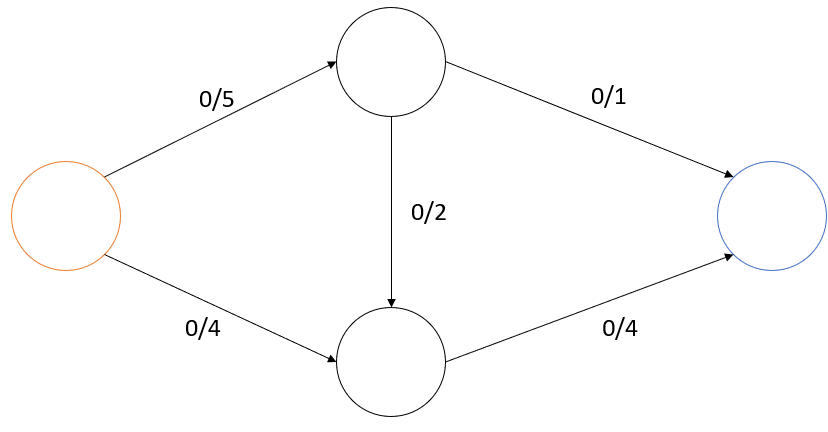
\includegraphics[scale=0.5]{pics/dop29_1.png}

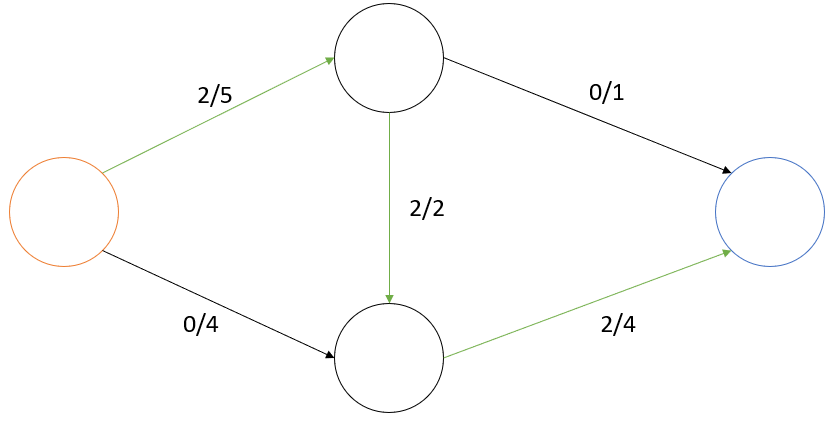
\includegraphics[scale=0.5]{pics/dop29_2.png}

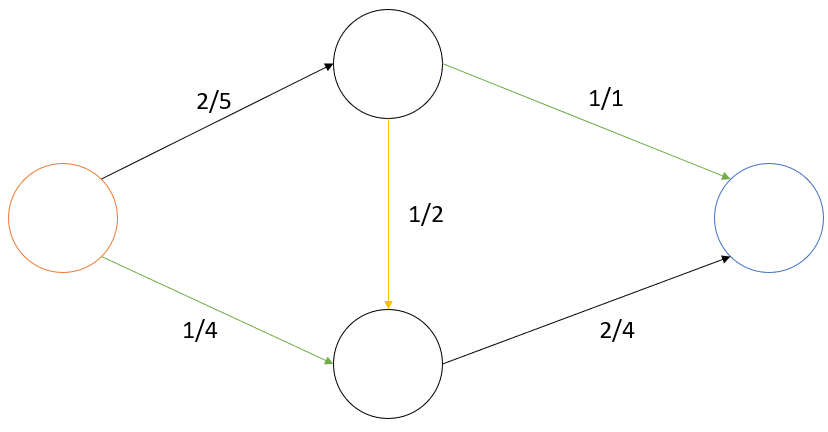
\includegraphics[scale=0.5]{pics/dop29_3.png}

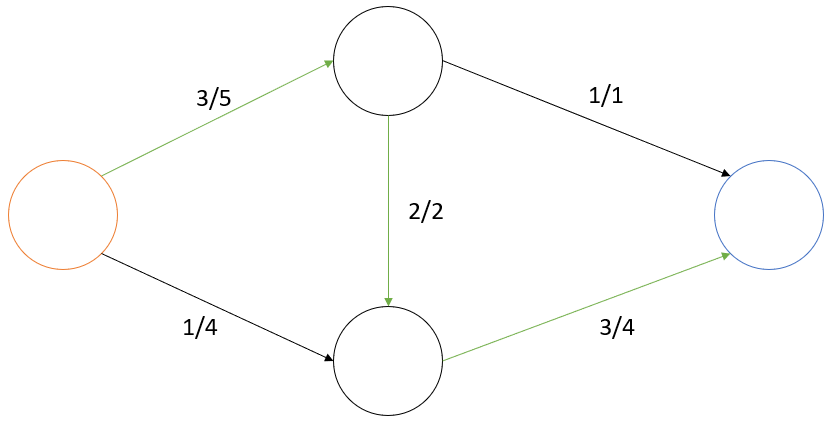
\includegraphics[scale=0.5]{pics/dop29_4.png}

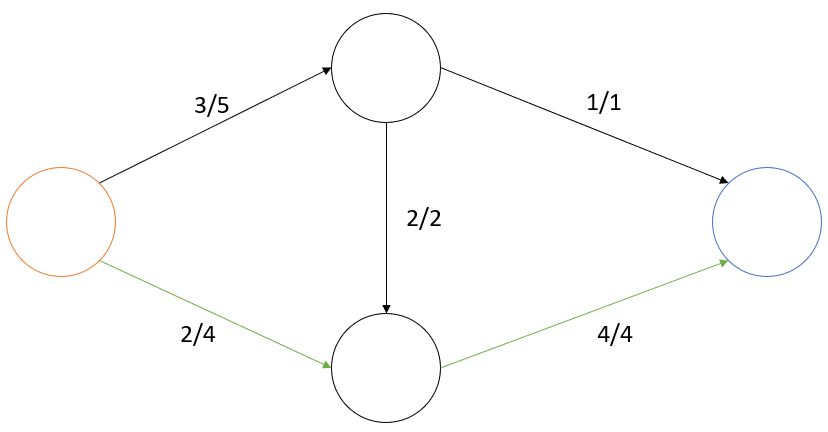
\includegraphics[scale=0.5]{pics/dop29_5.png}

% -------- source --------
\bigbreak
[\cite[page 69-96]{replace_me}]